\setcounter{framenumber}{0}

\section{Introduction}
\label{sec:intro}

\begin{frame}{Model Order Reduction (MOR)}
  \begin{figure}
    \centering
    \visible<1>{%
      \animategraphics[autoplay,loop,width=0.8\linewidth]{10}{images/frames/frame_}{000}{100}%
    }
    \caption*{\tiny McQuarrie, Huang, \& Willcox (2021). \textit{Data-driven reduced-order models via regularised operator inference for a single-injector combustion process}.}
  \end{figure}

  \uncover<2>{
    \vspace{-0.23cm}
    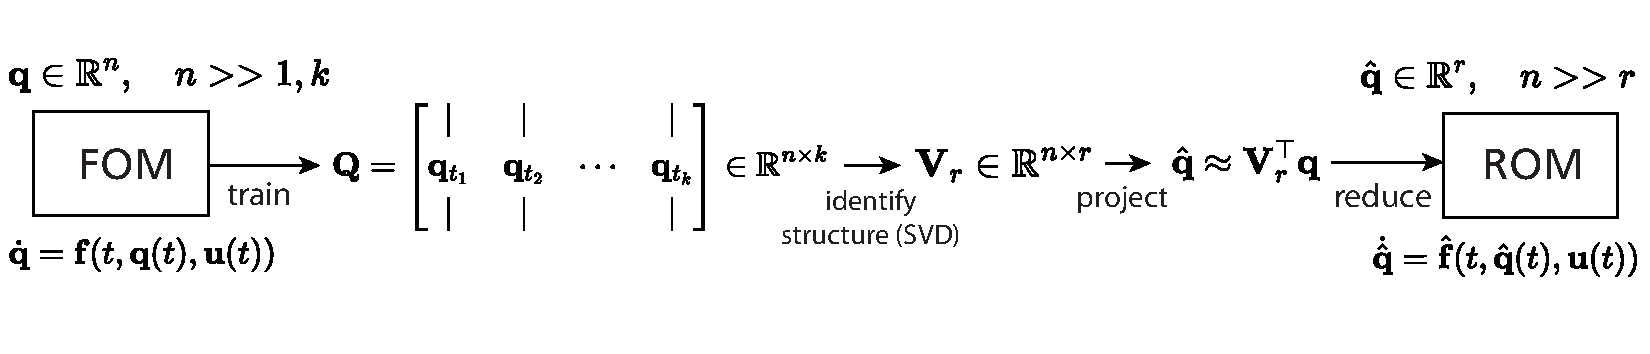
\includegraphics[width=\textwidth]{images/mor.pdf}
  }
\end{frame}


\begin{frame}{MOR Approaches}

\textbf{Example}: 1D - Viscous Burgers' Eq.

\[
  \frac{\partial}{\partial t}q(x,t)
  = \nu \frac{\partial^2}{\partial x^2}q(x,t)
    \;-\;\frac{\partial}{\partial x}
      \frac{q(x,t)^2}{2}
  \;\xrightarrow{\text{Spatial Discr.}}\;
  \dot{\mathbf{q}}(t)
  = \mathbf{A}\,\mathbf{q}(t)
    + \mathbf{H}\bigl(\mathbf{q}(t)\otimes\mathbf{q}(t)\bigr)
\]
\vspace{-0.5cm}
\[
  \hspace{9.2cm}\bigl\downarrow\!\scriptstyle\text{MOR}\bigr.
\]
\[
  ~~~~~~~~~~~~~~~~~~~~~~~~~~~~~~~~~~~~~~~~~~~~~~~~~~~~~~~~~~~~~~~~~~~~~\dot{\hat{\mathbf{q}}}(t)
  = \hat{\mathbf{A}}\,\hat{\mathbf{q}}(t)
    + \hat{\mathbf{H}}\bigl(\hat{\mathbf{q}}(t)\otimes\hat{\mathbf{q}}(t)\bigr)
\]

\vspace{-0.3cm}
Within MOR we differentiate:
\vspace{0.1cm}
    \begin{itemize}
        \item \textcolor{codeblue}{\emph{Intrusive (projection-based) MOR:}} Requires explicit access to $\mathbf{c}$, $\mathbf{A}$, $\mathbf{H}$, $\mathbf{B}$ so that the reduced order operators can be assembled:{\small
        $$\mathbb{R}^r \ni\hat{\mathbf{c}}=\mathbf{V}_r^{\top}\mathbf{c},~~\mathbb{R}^{r\times r} \ni\hat{\mathbf{A}}=\mathbf{V}_r^{\top}\mathbf{A}\mathbf{V}_r^{},~~\mathbb{R}^{r\times r^2} \ni\hat{\mathbf{H}}=\mathbf{V}_r^{\top}\mathbf{H(\mathbf{V}_r^{}\otimes\mathbf{V}_r^{\top})},~~\mathbb{R}^{r\times m} \ni\hat{\mathbf{B}}=\mathbf{V}_r^{\top}\mathbf{B},$$}
        \item \textcolor{codeblue}{\emph{Non-intrusive (data-driven) MOR:}} Does not explicitly project $\mathbf{c}$, $\mathbf{A}$, $\mathbf{H}$, and $\mathbf{B}$. Instead, one gathers time-series data (snapshots of $\mathbf{q}(t)$ and, if needed, $\dot{\mathbf{q}}(t)$), projects onto $\mathbf{V}_r$, and learns reduced operators by regression.
    \end{itemize}
  
\end{frame}